\chapter{Einleitung}

\begin{itemize}
    \item Schüttgutsortierung ist ein wichtiges Thema \todo{hier vielleicht dieses 10\% der Energie Beispiel bringen?}
    \item Anwendungsbereiche Schüttgutsortierung
    \item Maschinelle Lernverfahren sind ein heißes Thema, dass bei vielen existierenden problemen Anwendung findet
\end{itemize}

Schüttgüter und ihr Transport sind aus unserer modernen, globalisierten Welt nicht mehr wegzudenken.
Ob es sich um Lebensmittel wie Getreide, Kaffeebohnen oder Zucker, Bergbauerzeugnisse wie Eisenerze oder Kohle, oder [Granulat/Pellets] handelt, 
[...]
[nicht-destruktiv]
In dieser Arbeit soll es insbesondere um die bilddatenbasierte beziehungsweise optische Schüttgutsortierung gehen.



\todo{Einleitungstext}

\section{Motivation}

\color{blue}
\begin{itemize}
    \item State of the Art: große Sortierer 
    \item Kooperation ISAS IOSB, \textit{TrackSort} Projekt 
    \item Flächenkamera
    \item 2 geteiltes Problem: Tracking und Prediction
    \item Fokus dieser Arbeit: Prediction
    \item Bewegungsmodelle für verschiedene Schüttgüter von Hand finetunen ist viel Aufwand und schwer
    \item Option: Neuronale Netze einsetzen! 
    \item zwei verschiedene Problemstellungen:
    \item 1. die Position des Teilchens im nächsten Zeitschritt. \textbf{NextStep} für Trackingphase
    \item 2. die Position (und die Zeit) die das Teilchen beim Passieren des Düsenarrays haben wird. \textbf{Separator}
    \item Aktuell: auf Messungen - kein Vollständiger Schätzer
\end{itemize}
\color{black}

\todo[inline]{arbeit motivieren. Schüttgutsortierung ist ein interessantes Feld, das sich potenziell für ML anbietet.}
\todo[inline]{auf jeden fall separator- und NextStep-Netze unterscheidung erwähnen}

Der Großteil der heute in der Industrie eingesetzten optischen Schüttgutsortierer verwenden Zeilenkameras.
Dabei muss jedoch die Annahme getroffen werden, dass die Schüttgutpartikel keinerlei Geschwindigkeit orthogonal zur Transportrichtung haben,
weil diese nicht erfasst werden kann.
In Abbildung~\ref{fig:predMissed} ist dargestellt wie es zu einer Fehlseparierung kommen kann, wenn diese Annahme verletzt wird.
Durch den Einsatz von Flächenkameras ist es möglich, die Position eines Partikels auf dem Förderband zu mehreren Zeitpunkten zu bestimmen.
Basierend auf diesen Informationen sollen die Trajektorien der einzelnen Partikel vorhergesagt werden.
Diese sollen dazu verwendet werden, um die Sortierqualität zu steigern. 
Im Rahmen des \textit{TrackSort} Projekts, 
einer Kooperation zwischen dem Lehrstuhls für Intelligente Sensor-Aktor-Systeme (ISAS) des Karlsruher Instituts für Technologie
und dem Fraunhofer-Institut für Optronik, Systemtechnik und Bildauswertung (IOSB), 
wurde die Verbesserung der Schüttgutsortierung durch den Einsatz von Trackingverfahren betrachtet.
\todo[inline]{passt das hier rein, oder soll ich das eher wo anders erwähnen?}

\begin{figure}[h]
    \centering
    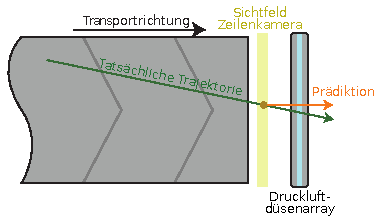
\includegraphics[width=0.8\textwidth]{PredictionMissed_translated.pdf}
    \caption{Darstellung einer Fehlseparierung durch die Annahme, dass es keine Bewegung orthogonal zur Transportrichtung gibt. 
    Übersetzt aus~\cite{Pfaff2018}.}
    \label{fig:predMissed}
\end{figure}


Um die zukünftigen Trajektorien der Partikel aus den vergangenen Positionen vorherzusagen, existieren verschiedene Bewegungsmodelle.
Diese liefern für unterschiedliche Situationen, mit unterschiedlichen Bandgeschwindigkeiten, Schüttguttypen oder Prädiktionsdistanzen, unterschiedlich gute Ergebnisse.  
Mittels neuronaler Netze können komplexe, nichtlineare Muster aus bestehenden Daten gelernt werden, ohne dass explizit auf diese hingewiesen werden müssen.
Es ist also denkbar, dass sie in der Lage wären die Bewegungen des Schüttguts zu lernen.
Die für den Einsatz von neuronalen Netzen essenziellen Daten in ausreichender Menge zu sammeln ist definitiv möglich. 
In dieser Arbeit soll nun erforscht werden, inwiefern der Einsatz von neuronalen Netzen zu einer Verbesserung gegenüber den bestehenden Ergebnissen führen kann.
Dabei wird exemplarisch mit Daten von dem \textit{TableSort} Schüttgutsortier gearbeitet.

Dafür sollen im Rahmen dieser Arbeit zwei verschiedene Prädiktionsprobleme durch neuronale Netze gelöst werden.
Einerseits soll vorhergesagt werden, an welcher Position sich ein Teilchen im nächsten Zeitschritt befinden wird.
Solche Netze werden von hier an als NextStep-Netze bezeichnet.
Eine Visualisierung dieser Aufgabe ist in Abbildung~\ref{fig:visualsNextstep} zu sehen.
Dies hilft dabei, das Zuordnungsproblem bei Multi-Target-Tracking zu lösen.
Andererseits soll vorhergesagt werden, an welcher Position und wann ein Teilchen das Druckluftdüsenarray passieren wird.
Diese Problemstellung wird von sogenannten Separator-Netzen gelöst.
Eine Visualisierung dieser Aufgabe ist in Abbildung~\ref{fig:visualsSeparator} zu sehen.
Die Qualität dieser Prädiktion ist ausschlaggebend für den Erfolg der Separation.


\begin{figure}[p]
    \centering
    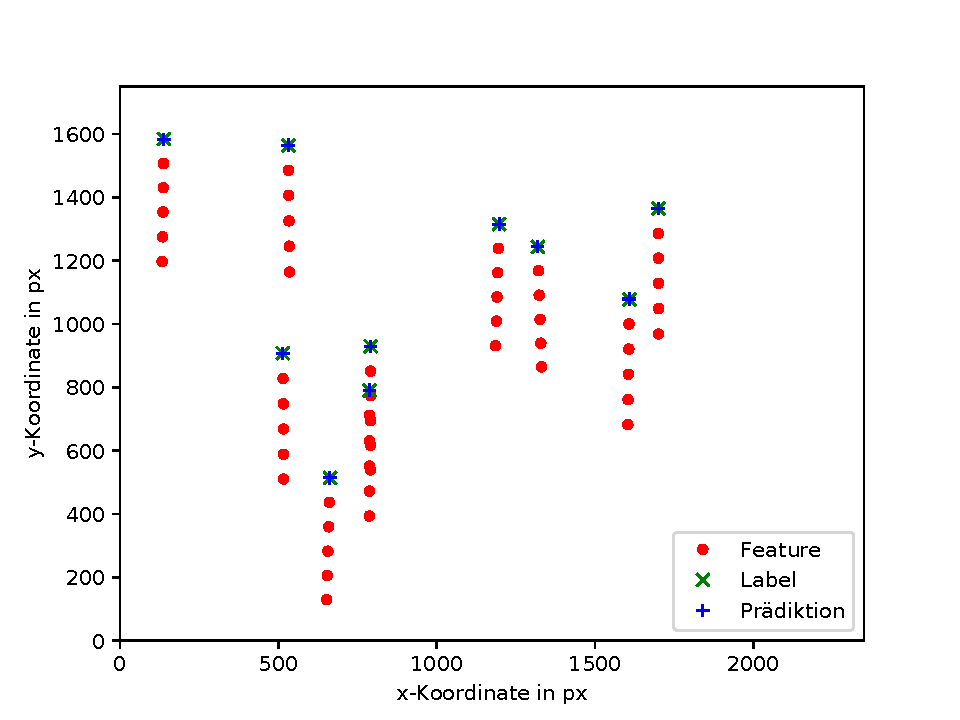
\includegraphics[width=0.8\textwidth]{NextStep-45kDecaySteps-ZylinderReal_2018-11-29.pdf}
    \caption[Visualisierung einer gelösten Probleminstanz eines NextStep-Netzes]{Visualisierung einer gelösten 
    Probleminstanz eines NextStep-Netzes. Die Transportrichtung ist entlang der \(y\)-Achse nach oben.
    Die Features sind die zeitlich aufeinanderfolgenden, beobachteten Positionen eines Partikels.
    Das Label ist die Position des entsprechenden Partikels im nächsten Zeitschritt.
    }
    \label{fig:visualsNextstep}
\end{figure}


\begin{figure}[p]
    \centering
    % \missingfigure{Real_Weizen_final_separatorExample.pdf}
	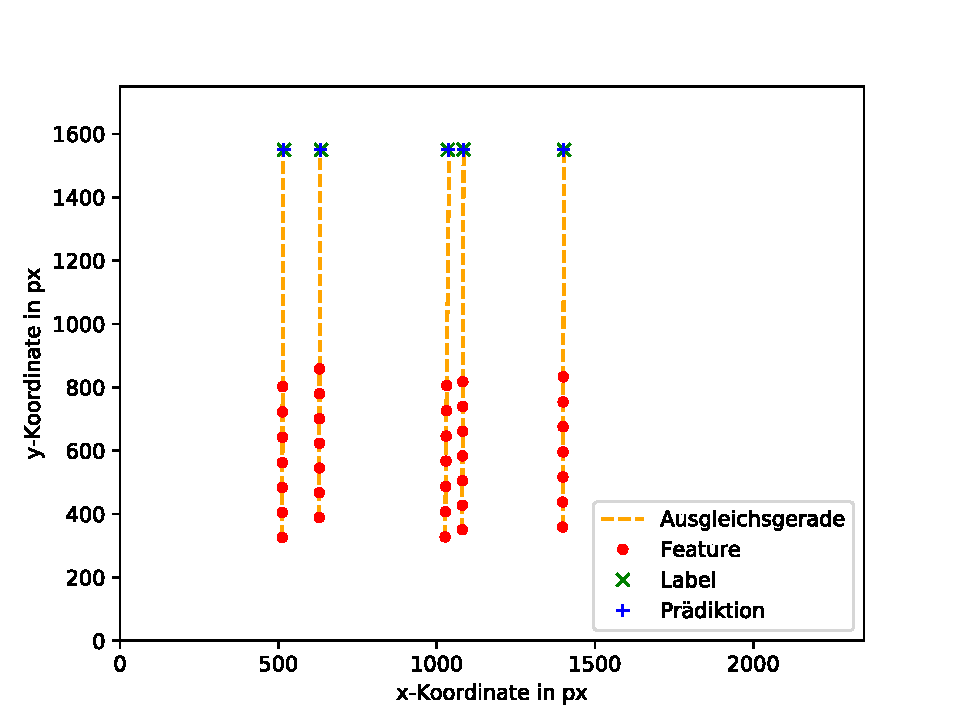
\includegraphics[width=0.8\textwidth]{Real_Weizen_final_separatorExample.pdf}
    \caption[Visualisierung einer gelösten Probleminstanz eines Separator-Netzes]{Visualisierung einer gelösten Probleminstanz 
    eines Separator-Netzes.
    Wie in Abbildung~\ref{fig:visualsNextstep} ist die Transportrichtung entlang der \(y\)-Achse nach oben.
    Die Features sind erneut die zeitlich aufeinanderfolgenden, beobachteten Positionen eines Partikels.
    Das eine Element des Label ist die Position entlang der \(x\)-Achse an der das entsprechende Partikel das Druckluftdüsenarray passiert.
    Das zweite Element des Labels -- der Zeitpunkt an dem es das Druckluftdüsenarray passiert -- ist nicht abgebildet.
    }
	
	\label{fig:visualsSeparator}
\end{figure}



\section{Aufbau der Arbeit}

Das schreibe ich auf, wenn die Gliederung finalisiert ist.

\todo{aufbau Gliederung beschreiben. Ganz am Ende dann, wenn sich nichts mehr ändert}

